% chessforensics.tex — Bayesian Chess Cheat Detection
% Compile: pdflatex paper.tex && bibtex paper && pdflatex paper.tex && pdflatex paper.tex
\documentclass[11pt,a4paper]{article}

% ── Packages ──────────────────────────────────────────────────────────────────
\usepackage[utf8]{inputenc}
\usepackage[T1]{fontenc}
\usepackage{amsmath,amsthm,amssymb}
\usepackage[expansion=false]{microtype}
\usepackage{mathtools}
\usepackage{booktabs}
\usepackage{multirow}
\usepackage{graphicx}
\usepackage[margin=2.5cm]{geometry}
\usepackage{hyperref}
\usepackage{cleveref}
\usepackage{algorithm}
\usepackage{algpseudocode}
\usepackage{natbib}
\usepackage{xcolor}
\usepackage{enumitem}
\usepackage{subcaption}

\hypersetup{
  colorlinks=true,
  linkcolor=blue!70!black,
  citecolor=green!50!black,
  urlcolor=blue!60!black,
}

% ── Math operators ────────────────────────────────────────────────────────────
\DeclareMathOperator{\logit}{logit}
\DeclareMathOperator{\sigmoid}{sigmoid}
\DeclareMathOperator*{\argmax}{arg\,max}
\DeclareMathOperator*{\argmin}{arg\,min}
\DeclareMathOperator{\Var}{Var}
\DeclareMathOperator{\Cov}{Cov}
\DeclareMathOperator{\diag}{diag}
\newcommand{\dB}{\,\mathrm{dB}}
\newcommand{\given}{\,|\,}
\newcommand{\R}{\mathbf{R}}
\newcommand{\z}{\mathbf{z}}
\newcommand{\w}{\mathbf{w}}
\newcommand{\bmu}{\boldsymbol{\mu}}

\theoremstyle{definition}
\newtheorem{definition}{Definition}

% ══════════════════════════════════════════════════════════════════════════════
\title{%
  \textbf{ChessForensics: Bayesian Detection of Engine Assistance\\
  in Competitive Chess}%
}
\author{%
  Alberto Mirandola%
}
\date{November 2026}

\begin{document}
\maketitle

% ══════════════════════════════════════════════════════════════════════════════
\begin{abstract}
I present a statistical framework for detecting engine assistance in
competitive chess.  The core innovation is a \emph{per-move log-likelihood
ratio}: for each position, a logistic regression model fitted on the
training corpus predicts the probability that an honest player matches
the engine's top choice given position-specific features (evaluation gap,
legal move count, complexity, and spread).  This position-specific
probability feeds a binary log-LR that is summed across moves and
integrated over four assistance rates
$r \in \{10\%, 25\%, 50\%, 100\%\}$ via a mixture model.
Multi-game evidence uses a per-player mixture that charges the
model-selection penalty once.  Per-band null calibration ensures
uniform false-positive rates across rating levels.

Training and evaluation data are strictly separated.  Thresholds
are selected on 28{,}670 out-of-sample Chess.com games (V1,
15{,}586 players) and tested on a held-out set of 22{,}932 games
(V2, 7{,}505 players, zero overlap).  Using band-stratified
thresholds, V2's false-positive rate is at or below the target at
every level tested (e.g.\ 0.47\% at a 1\% target in the 2000--2200
band; 95\% CI $[0.38, 0.58]\%$).
All ten FIDE-sanctioned cheating cases tested produce positive aggregate
evidence ($+4.7$ to $+55.6\dB$); eight exceed $+10\dB$.

A pre-registered head-to-head comparison against four baselines
(including a Regan-style two-signal approach) on 5{,}000 held-out
games with paired McNemar tests shows the per-move model achieves
87\% per-player detection at 1\% FPR for 25\%-rate assistance (vs
64\% for the Regan-style baseline, $p < 10^{-42}$), while correctly
clearing Kasparov's ``immortal game'' ($-4.9\dB$) that the
Regan-style baseline would flag ($+8.4\dB$).
\end{abstract}

\medskip
\noindent\textbf{Keywords:} chess, cheating detection, Bayesian inference,
log-likelihood ratio, choice model, engine assistance, fair play.

% ══════════════════════════════════════════════════════════════════════════════
\section{Introduction}
\label{sec:intro}

The availability of superhuman chess engines on commodity hardware poses a
serious and growing threat to competitive chess integrity.  A player
who secretly consults an engine---even on a small fraction of
moves---gains a decisive advantage that is invisible to opponents and
arbiters.  High-profile cases, from Borislav Ivanov's implausible
results at the 2012 Zadar Open to the Carlsen--Niemann controversy at
the 2022 Sinquefield Cup, have underscored the need for rigorous
statistical methods.

The foundational work is due to
Regan~\citep{regan2011understanding,regan2014cheating}, who introduced
the multinomial choice model that maps engine evaluations to expected
move probabilities, then tests whether a player's accuracy is
statistically anomalous.  The present system builds on Regan's framework with
several extensions:

\begin{enumerate}[nosep]
  \item \textbf{Per-move log-likelihood ratios.}  Rather than
    aggregating moves into a single game-level z-score, the system
    computes a binary log-LR for each move using a position-specific
    probability of matching the engine's top choice.  This
    probability comes from a per-band logistic regression on six
    position features (evaluation gap, legal move count, complexity,
    spread, gap-small indicator, only-move indicator), fitted on
    2.7~million training games (AUC $\approx$ 0.75).
  \item \textbf{Four-rate mixture model} over assistance levels
    $r \in \{10\%,25\%,50\%,100\%\}$.  Per-move log-LRs are computed
    separately for each rate and combined via $\mathrm{logsumexp}$,
    enabling detection of partial or intermittent engine use without
    requiring the rate to be specified in advance.
  \item \textbf{Per-band null calibration} that z-normalises the raw
    dB score against each rating band's honest distribution, ensuring
    uniform false-positive rates across rating levels.
  \item \textbf{Per-player aggregation} that sums per-rate log-LRs
    across games and applies the mixture penalty once, dramatically
    improving multi-game detection of partial cheating.
  \item \textbf{Fifteen supplementary signals} spanning move accuracy,
    error distribution shape, clock behaviour, and engine
    fingerprinting, available for display and secondary analysis.
\end{enumerate}

The remainder of this paper is organised as follows.
\Cref{sec:related} reviews related work.
\Cref{sec:model} presents the choice model and signal definitions.
\Cref{sec:pipeline} describes the end-to-end analysis pipeline.
\Cref{sec:calibration} describes null calibration.
\Cref{sec:evidence} details the Bayesian evidence framework.
\Cref{sec:data} describes corpus construction and train/test separation.
\Cref{sec:validation} reports validation results.
\Cref{sec:synthetic} presents a pre-registered head-to-head comparison
against four baselines.
\Cref{sec:discussion} discusses limitations, and
\Cref{sec:conclusion} concludes.

% ══════════════════════════════════════════════════════════════════════════════
\section{Related Work}
\label{sec:related}

Regan and Haworth~\citep{regan2011understanding} introduced the
\emph{intrinsic performance rating} (IPR), estimating a player's
strength from the sensitivity parameter of a multinomial logit model
fitted to engine evaluations.  Regan~\citep{regan2014cheating}
subsequently developed a hypothesis-testing framework comparing observed
match rates against expected rates under a Poisson-binomial model,
applying this methodology as a consultant for FIDE's Anti-Cheating
Commission.

Other approaches include na\"ive centipawn-loss thresholds
\citep{guid2006computer}, which suffer from position-complexity
confounding and lack formal error control;
large-scale historical analyses using aggregate
statistics~\citep{alliot2017who,ferreira2013using}; move-matching
percentages without per-position calibration; and machine-learning
classifiers trained on labelled data, which risk overfitting to
specific engine versions.

This work differs in two key respects.  First, instead of testing
aggregate game-level statistics, I compute a \emph{per-move}
log-likelihood ratio using position-specific match probabilities from a
fitted logistic model, which preserves position-level information that
game-level z-scores discard.  Second, the per-move log-LRs are
integrated over a four-rate mixture model for partial assistance, with
per-band null calibration from a 3.4-million-game corpus under strict
train/test separation.  I validate against ten FIDE-sanctioned cheating
cases with known ground truth, 28{,}670 out-of-sample Chess.com games,
and a pre-registered head-to-head comparison against Regan-style
baselines with paired statistical tests.


% ══════════════════════════════════════════════════════════════════════════════
\section{The Choice Model and Signal Extraction}
\label{sec:model}

\subsection{Multinomial Choice Model}
\label{sec:choice}

Given a position with $K$ legal moves ranked by engine evaluation, let
$\delta_i \ge 0$ denote the evaluation loss (in pawns) of move~$i$
relative to the best move ($\delta_1 = 0$).  The probability that a
player of sensitivity~$s > 0$ and consistency~$c > 0$ plays move~$i$ is
\begin{equation}
  \label{eq:choice}
  P(i \given s, c)
  = \frac{\exp\!\bigl(-(\delta_i / s)^c\bigr)}
         {\sum_{j=1}^{K} \exp\!\bigl(-(\delta_j / s)^c\bigr)},
\end{equation}
a softmax (multinomial logit) model~\citep{regan2011understanding}
where smaller~$s$ corresponds to stronger play (finer sensitivity to
evaluation differences) and larger~$c$ implies sharper discrimination
between small and large errors.

\paragraph{Tail extrapolation.}
Engine analysis returns the top $k$ moves (MultiPV${}=5$).  For the
remaining $K - k$ legal moves, I extrapolate evaluation losses
linearly: $\delta_{k+j} = \delta_k + j \cdot \Delta$, where
$\Delta = \max(0.05, \delta_k - \delta_{k-1})$, clipped at
$\delta_{\max} = 6.0$~pawns.  This prevents upward bias in the fitted~$s$
by maintaining the proper normaliser.

\paragraph{Maximum-likelihood estimation.}
Parameters $(s, c)$ are fitted by maximising the log-likelihood
\begin{equation}
  \label{eq:loglik}
  \ell(s,c) = \sum_{m=1}^{n} \log P\bigl(\text{played}_m \given s, c\bigr)
\end{equation}
over $n$ scoreable positions, using L-BFGS-B~\citep{byrd1995limited} in log-space
$(\log s, \log c)$ with multiple restarts.  Standard errors are obtained
from the observed Fisher information (numerical Hessian) and
back-transformed via the delta method:
$\mathrm{SE}_s = s \sqrt{\widehat{\Var}[\log s]}$.

\paragraph{Intrinsic Performance Rating (IPR).}
A calibration curve $\{(\bar{E}_b, \tilde{s}_b)\}_{b=1}^{B}$ maps each
rating band's median fitted~$s$ to its midpoint Elo $\bar{E}_b$.
Monotonicity is enforced via isotonic regression (pool-adjacent-violators
algorithm).  For a subject game with fitted $\hat{s}$, the IPR is
obtained by log-linear interpolation:
\begin{equation}
  \label{eq:ipr}
  \widehat{\mathrm{Elo}}
  = \mathrm{interp}\!\bigl(\log \hat{s};\;
      \{\log \tilde{s}_b\},\; \{\bar{E}_b\}\bigr).
\end{equation}
Confidence intervals propagate $\mathrm{SE}_s$ through the same
interpolation.  The curve is validated on the 12 band midpoints
(\Cref{sec:validation}).

% ──────────────────────────────────────────────────────────────────────
\subsection{Match-Rate Signals}
\label{sec:matchrate}

For each scoreable position~$m$, the reference model yields per-position
match probabilities $p_m^{(1)}, p_m^{(2)}, p_m^{(3)}$ for agreeing with
the engine's top-1, top-2, and top-3 moves respectively.  The observed
match count $X = \sum_m \mathbf{1}[\text{matched}]$ follows a
\emph{Poisson-binomial} distribution~\citep{hong2013computing} with
heterogeneous success probabilities, for which exact computation is
available via $O(n^2)$ dynamic programming.

\begin{definition}[Match-rate z-score]
\begin{equation}
  \label{eq:matchz}
  z_{\mathrm{t}k} = \frac{X_k - \sum_m p_m^{(k)}}
    {\sqrt{\sum_m p_m^{(k)}(1 - p_m^{(k)})}},
  \qquad k \in \{1,2,3\}.
\end{equation}
\end{definition}

The exact one-sided $p$-value $\Pr(X_k \ge x_k)$ is computed from the
Poisson-binomial PMF; the mid-$p$ variant
$\Pr(X_k > x_k) + \tfrac{1}{2}\Pr(X_k = x_k)$ is used to reduce
conservatism.

% ──────────────────────────────────────────────────────────────────────
\subsection{Accuracy Signals}
\label{sec:acpl}

\paragraph{Average centipawn loss (ACPL).}
Let $\delta_m^{\mathrm{cp}}$ denote the centipawn loss on move~$m$.
Under the reference model, the per-position expected loss
$\mu_m = \mathbb{E}[\delta^{\mathrm{cp}}_m]$ and variance
$\sigma_m^2 = \Var[\delta^{\mathrm{cp}}_m]$ are computed from the
multinomial choice probabilities.  The ACPL signal tests whether the
observed mean loss is anomalously low:
\begin{equation}
  \label{eq:acplz}
  z_{\mathrm{acpl}}
  = \frac{\bar{\delta}^{\mathrm{cp}} - \bar{\mu}}
         {\sqrt{\sum_m \sigma_m^2 / n^2}},
\end{equation}
where lower (more negative) $z$ indicates suspiciously accurate play.

\paragraph{Accuracy--complexity slope.}
A logistic regression of $\mathrm{matched\_t1}$ on position complexity
yields a slope; stronger players (and engines) maintain accuracy even on
complex positions.  The slope z-score tests whether the observed slope
is anomalously flat relative to the band reference.

\paragraph{CPL--complexity slope.}
Analogously, a linear regression of centipawn loss on complexity yields
a slope; engine-assisted play shows unnaturally constant CPL across
complexity levels.

\paragraph{CPL tail test.}
Rather than testing the mean, this signal tests whether the blunder
distribution is suspiciously \emph{truncated}---i.e., whether large
errors are missing.  Per position, the probability of a blunder
exceeding threshold $\beta$ (default 200\,cp) is
\begin{equation}
  P(\text{blunder}_m) = 1 - \Phi\!\left(\frac{\beta - \mu_m}{\sigma_m}\right).
\end{equation}
The observed blunder rate is compared to the expected rate via a
variance-weighted z-test, with sign inverted so that fewer blunders
yields positive~$z$.

% ──────────────────────────────────────────────────────────────────────
\subsection{Timing Signals}
\label{sec:timing}

Clock data, when available, provides signals orthogonal to move quality.
Each timing signal carries a validity weight
$w_{\mathrm{speed}} \in [0, 1]$ that depends on time control:
classical receives full weight ($w = 1.0$), rapid $w = 0.75$, blitz
$w = 0.30$, bullet $w = 0.05$, and correspondence $w = 0$.

\paragraph{Time--complexity correlation.}
Honest players spend more time on complex positions.  The Spearman rank
correlation $\rho$ between think times and position complexity is
computed; $z_{\mathrm{rho}} = -\rho / \mathrm{SE}_\rho$, so that low
correlation (engine-like uniform speed) yields positive~$z$.

\paragraph{Residual coefficient of variation.}
After regressing $\log(\text{time})$ on complexity, the standard
deviation of residuals measures timing uniformity.  Lower residual CV
(more robotic timing) is suspicious.

\paragraph{Cadence detection.}
A modal-clustering analysis identifies the fraction of moves within
$\pm 0.35$\,s of the most common think time.  High cadence fraction
(e.g., consistently playing on the increment) is suspicious.

\paragraph{Timing--accuracy cross-signal.}
Among high-complexity positions (top 40\%) where the player matched the
engine's top move, the mean think time is compared to the band baseline.
Suspiciously fast correct play on hard positions is flagged via a
log-space z-test.

% ──────────────────────────────────────────────────────────────────────
\subsection{Structural Signals}
\label{sec:structural}

\paragraph{Switchpoint detection.}
A two-rate binomial likelihood-ratio scan tests whether a player's
accuracy undergoes a sudden jump mid-game, consistent with starting
engine consultation after an initial honest phase.  For each candidate
split point~$k$ (with minimum segment length 8), I compute
\begin{equation}
  \Lambda_k
  = \ell(\hat{p}_{\mathrm{before}}, \hat{p}_{\mathrm{after}})
  - \ell(\hat{p}_{\mathrm{all}}),
\end{equation}
where $\hat{p}$ are the MLE binomial rates.  The best split
$k^* = \argmax_k \Lambda_k$ is tested via 2{,}000 permutations,
requiring both $p < 0.05$ and a rate jump exceeding 18 percentage
points.  The z-score is the probit transform of the permutation
$p$-value, boosted by a factor of 1.3 when the player was losing at the
switchpoint.

\paragraph{IPR gap.}
The difference between the intrinsic performance rating and the player's
nominal Elo, normalised by the estimated single-game IPR standard
deviation ($\approx 250$~Elo), provides a signal that is strongest for
lower-rated players receiving full engine assistance.

\paragraph{Engine fingerprinting.}
When a second engine (e.g., Leela Chess Zero at low depth) is available,
the \emph{deep-only match rate}---agreement with the primary engine on
positions where the second engine disagrees---isolates engine-specific
move selection patterns that honest players are unlikely to replicate.

% ══════════════════════════════════════════════════════════════════════════════
\section{Analysis Pipeline}
\label{sec:pipeline}

A game is processed through the following stages:

\paragraph{1.\ Engine analysis (three passes).}
Every position is first analysed at depth~4/MultiPV~3 (``L0''), which
identifies moves that any shallow search would find.  A depth-12/MultiPV-5
pass then scores all positions.  A priority ranker flags critical
positions---where the played move diverges from the engine's top choice,
where the evaluation swings, or where the position is tactically
complex---and promotes them to a depth-22/MultiPV-5 deep pass, up to a
budget of $\sim$40\% of total plies.  This adaptive schedule concentrates
compute on the positions that carry forensic information.

\paragraph{2.\ Position filtering.}
Positions are excluded from scoring if they fall within detected book
lines or are forced (one legal move).  Positions with evaluation beyond
$\pm 6$~pawns are also excluded---not because cheating is impossible
there, but because the choice model's discriminative power vanishes:
when any reasonable move wins, the expected top-1 match rate approaches
100\% for honest players and cheaters alike, so including these
positions adds noise without signal.  A minimum of 8 scoreable
positions is required; games below this threshold receive no verdict.

\paragraph{3.\ Feature extraction.}
For each scoreable position, the system records: whether the played move
matches the engine's top-1/2/3 choices, the centipawn loss, the position
complexity (number of reasonable alternatives weighted by evaluation
spread), clock time consumed, and the L0 agreement flag.  These per-move
features are assembled into a DataFrame from which game-level signals
are computed.

\paragraph{4.\ Signal computation.}
Fifteen signals are extracted (\Cref{app:signals}): three match-rate
z-scores via Poisson-binomial tests, an ACPL z-score, two
accuracy-vs-complexity slopes, a CPL tail test, a switchpoint scan, an
IPR gap, four timing signals (including a timing--accuracy
cross-signal), and two engine-fingerprint signals (when a second
engine is available).

\paragraph{5.\ Per-move scoring and evidence combination.}
For each scoreable position, a per-band logistic regression predicts the
probability of matching the engine's top choice.  A binary log-LR is
computed per move and summed across positions, integrated over four
assistance rates via the mixture model, and calibrated against the
band's honest null distribution (\Cref{sec:evidence}).
A Monte Carlo sensitivity band (4{,}000 draws) quantifies how the
posterior moves under model uncertainty.

\paragraph{6.\ Multi-game aggregation.}
When multiple games from the same player are available, per-rate log-LRs
are summed across games and the mixture penalty is applied once
(\Cref{sec:multigame}).  The aggregate posterior and per-game
evidence breakdown constitute the final verdict.


% ══════════════════════════════════════════════════════════════════════════════
\section{Null Calibration}
\label{sec:calibration}

Raw z-scores from the hypothesis tests of \Cref{sec:model} exhibit
systematic bias and overdispersion relative to the standard normal, due
to model misspecification and the simplifying assumptions of the choice
model.  These are corrected via a three-tier calibration scheme.

\paragraph{Tier 1: Per-band calibration.}
For each of 12 rating bands (width 200 Elo, from 800--1000 to
2800+), the empirical mean (bias $b_{\mathrm{band}}$) and
standard deviation (scale $\sigma_{\mathrm{band}}$) of each signal's
z-scores on the corpus of honest games within that band.  The corrected
z-score is
\begin{equation}
  \label{eq:calib}
  z_{\mathrm{cal}} = \frac{z_{\mathrm{raw}} - b_{\mathrm{band}}}
    {\sigma_{\mathrm{band}}}.
\end{equation}

\paragraph{Tier 2: Pooled calibration.}
When the target band has insufficient data for a particular signal, the
system falls back to the pooled bias and scale computed across all bands
(e.g., ACPL: $b = 0.27$, $\sigma = 1.99$ from 70{,}948 player-games).

\paragraph{Tier 3: Empirical defaults.}
When no corpus calibration is available (e.g., a baseline built without
clock data), hardcoded empirical values are used.  These were measured
once on a large sample and serve as a fallback
(e.g., $\mathrm{time\_uniformity}$: $b = -0.09$, $\sigma = 1.40$).
The Tier~3 values for accuracy signals (e.g., $\mathrm{t1\_match}$:
$b = -0.51$, $\sigma = 1.66$) are more conservative than the
per-band Tier~1 values (typically $b \approx 0$,
$\sigma \approx 1.1$--$1.2$) because they pool across all ratings,
absorbing inter-band variance into a wider scale.

This three-tier design ensures graceful degradation: the system produces
calibrated posteriors even with incomplete baselines, while exploiting
the most specific calibration data when available.


% ══════════════════════════════════════════════════════════════════════════════
\section{Bayesian Evidence Combination}
\label{sec:evidence}

\subsection{Per-Move Log-Likelihood Ratio}
\label{sec:permove}

The central innovation of this system is a \emph{per-move} scoring
mechanism.  Rather than summarising a game into aggregate statistics
(match rate, ACPL) and testing those, I compute a log-likelihood ratio
for each individual move, preserving position-level information.

For each scoreable position~$m$, let $t_m \in \{0,1\}$ indicate whether
the player matched the engine's top choice, and let $p_m$ denote the
position-specific probability that an honest player of the appropriate
rating would make this match.  Under the null (honest play), the
probability of the observed outcome is
\begin{equation}
  \label{eq:null-move}
  P(t_m \given H_0) = p_m^{t_m} (1-p_m)^{1-t_m}.
\end{equation}
Under the alternative at assistance rate~$r$ (the player consults the
engine on each move independently with probability~$r$):
\begin{equation}
  \label{eq:alt-move}
  P(t_m \given H_1, r) =
  \begin{cases}
    r + (1-r)\,p_m & \text{if } t_m = 1, \\
    (1-r)(1-p_m)   & \text{if } t_m = 0.
  \end{cases}
\end{equation}
The per-move log-LR at rate~$r$ is therefore:
\begin{equation}
  \label{eq:permove-lr}
  \ell_m(r) =
  \begin{cases}
    \log\!\bigl(r + (1-r)\,p_m\bigr) - \log p_m & \text{if } t_m = 1, \\
    \log(1-r) & \text{if } t_m = 0.
  \end{cases}
\end{equation}

\paragraph{Position-specific $p_m$ via logistic regression.}
The key to this approach is an accurate, well-calibrated estimate
of~$p_m$.  Rather than using the global Poisson-binomial
model (\Cref{sec:matchrate}), which assigns expected match rates
based on the choice model fitted to band-level data, I train a
per-band logistic regression~\citep{hosmer2013applied} on six position features:
\begin{equation}
  \label{eq:logistic}
  \logit(p_m) = \beta_0 + \beta_1 \log(1+g_m/100)
    + \beta_2 \log L_m + \beta_3 C_m + \beta_4 S_m
    + \beta_5 G_m + \beta_6 O_m,
\end{equation}
where $g_m$ is the evaluation gap (centipawns) between the top two
engine moves, $L_m$ the number of legal moves, $C_m$ the position
complexity, $S_m$ the evaluation spread among top candidates, $G_m$ the
fraction of candidates within 30\,cp of the best, and $O_m$ an
indicator for forced moves ($L_m \le 2$ or gap $> 3$~pawns).  A
separate logistic regression is fitted for each of 12 rating bands on
the training corpus (2.7~million games), achieving AUC $\approx 0.75$
with well-calibrated probability outputs.

\subsection{Mixture Model Over Assistance Rates}
\label{sec:mixture}

A cheater may not use the engine on every move.  Following the
finite-mixture framework~\citep{mclachlan2000finite}, I model four
assistance rates $r \in \mathcal{R} = \{0.10, 0.25, 0.50, 1.0\}$
with a uniform prior $\pi_r = 1/|\mathcal{R}|$.  The per-game log-LR
at rate~$r$ sums over all $n$ scoreable positions:
\begin{equation}
  \label{eq:game-rate-lr}
  \log \mathrm{LR}_{\mathrm{game}}(r)
  = \sum_{m=1}^{n} \ell_m(r).
\end{equation}
The marginal log-LR integrates over rates:
\begin{equation}
  \label{eq:mixture}
  \log \mathrm{LR}_{\mathrm{mix}}
  = \log \sum_{r \in \mathcal{R}} \pi_r \cdot \mathrm{LR}_{\mathrm{game}}(r)
  = \mathrm{logsumexp}\!\bigl(
      \{\log \mathrm{LR}_{\mathrm{game}}(r) + \log \pi_r\}_{r \in \mathcal{R}}\bigr).
\end{equation}

\subsection{Per-Band Null Calibration}
\label{sec:permove-cal}

The raw per-move dB score exhibits systematic band-dependent bias:
stronger players have higher baseline match rates, and the logistic
model, while well-calibrated within each band, does not perfectly
cancel rating effects across bands.  I correct this by z-normalising
against each band's honest distribution:
\begin{equation}
  \label{eq:band-cal}
  \mathrm{dB}_{\mathrm{cal}}
  = \frac{\mathrm{dB}_{\mathrm{raw}} - b_{\mathrm{band}}}
         {\sigma_{\mathrm{band}}}
    \cdot \sigma_{\mathrm{pool}} + b_{\mathrm{pool}},
\end{equation}
where $(b_{\mathrm{band}}, \sigma_{\mathrm{band}})$ are the mean and
standard deviation of honest dB scores in the target band, and
$(b_{\mathrm{pool}}, \sigma_{\mathrm{pool}})$ are the pooled
reference.  This ensures that a single global threshold achieves
uniform FPR across rating bands.

\subsection{Posterior Probability}
\label{sec:posterior}

With a base-rate prior $\pi_0 = 0.01$ (1\% prevalence of engine
assistance), the posterior is
\begin{equation}
  \label{eq:posterior}
  P(\text{cheating} \given \text{game})
  = \sigmoid\!\bigl(\logit(\pi_0) + \log \mathrm{LR}_{\mathrm{mix}}\bigr),
\end{equation}
where $\logit(p) = \log\frac{p}{1-p}$ and
$\sigmoid(x) = \frac{1}{1 + e^{-x}}$.  Evidence strength is also
reported in decibans~\citep{good1979studies}:
\begin{equation}
  \label{eq:decibans}
  \mathrm{dB} = \frac{10 \cdot \log \mathrm{LR}}{\ln 10}.
\end{equation}

\subsection{Sensitivity Band}

A Monte Carlo procedure (4{,}000 draws) perturbs the per-move $p_m$
predictions by their estimated uncertainty (5\% relative jitter when the
corpus exceeds 50 games, 10\% otherwise) and recomputes the posterior,
yielding a 5th--95th percentile band that reflects model uncertainty.

\subsection{Multi-Game Per-Player Aggregation}
\label{sec:multigame}

For $N$ games by the same player, the per-rate log-LRs are summed across games:
\begin{equation}
  \label{eq:perplayer}
  L_r = \sum_{g=1}^{N} \log \mathrm{LR}_g(r),
  \qquad
  \log \mathrm{LR}_{\mathrm{player}}
  = \mathrm{logsumexp}\!\bigl(\{L_r + \log \pi_r\}_{r}\bigr).
\end{equation}
This formulation assumes a \emph{single constant assistance rate} per
player across all games, which charges the mixture penalty
$\log |\mathcal{R}| \approx 6\dB$ exactly once rather than once per
game.  This is critical for detecting partial assistance: in the Feller
case (\Cref{sec:cases}), per-game analysis misses the signal, while
per-player aggregation yields $+20.8\dB$ (detected).

\subsection{Supplementary Signal-Level Scoring}
\label{sec:signal-scoring}

In addition to the per-move LR, the system computes fifteen game-level
signals (\Cref{app:signals}) spanning match rates, ACPL, accuracy
slopes, timing, switchpoint detection, IPR gap, and engine
fingerprinting.  These can be combined via a multivariate Gaussian
log-LR with correlation adjustment and NNLS projection (detailed in
\Cref{sec:synthetic} as baseline method M4).  The signal-level approach
is retained for display, secondary analysis, and comparison purposes,
but the per-move LR is the primary scoring mechanism for all operational
verdicts.


% ══════════════════════════════════════════════════════════════════════════════
\section{Corpus and Calibration Data}
\label{sec:data}

\subsection{Corpus Construction}

The reference corpus comprises 3{,}400{,}451 rated rapid and classical
games (6.78 million player-games, 229.6 million positions) drawn from
two sources: the Lichess open database~\citep{lichess2024database} supplies the
bulk of games in bands below Elo~2200, while TWIC (The Week in Chess)
OTB tournament archives~\citep{twic2024} supply the majority of games
in the 2200--2400 through 2800+ bands.  Collection filters:
\begin{itemize}[nosep]
  \item Minimum 20 plies per game.
  \item Maximum 300 Elo gap between opponents.
  \item Rated games only; no correspondence.
  \item Accounts flagged for terms-of-service violations excluded.
\end{itemize}

A deep engine pass (Stockfish 17~\citep{stockfish2024}, depth 22, MultiPV 5) was applied to
41{,}698 games (70{,}906 player-games, 3.36 million positions).  A
``lite'' pass incorporating Lichess server evaluations extended ACPL
statistics to 226 million positions.

\subsection{Rating Bands}

Twelve bands span the rating range: a catch-all below 800, ten bands
of width 200 Elo from 800--1000 through 2600--2800, and one open-ended
band above 2800.  Each band
stores the median choice-model parameters $(\tilde{s}_b, \tilde{c}_b)$,
expected match rates, ACPL distribution, accuracy--complexity slopes,
and timing baselines.  Per-band null calibration (\Cref{sec:calibration})
is computed from the games within each band.

\subsection{Train/Test Independence}
\label{sec:traintestsplit}

The corpus is partitioned into a training set (used for fitting the
choice model, computing per-band calibration, and estimating the
correlation matrix) and a held-out test set of 682{,}952 games used
exclusively for false-positive rate estimation and calibration
verification.  No test-set game contributes to any model parameter.
Out-of-sample titled-player games (5{,}560 games from 92 GM/IM/WGM
accounts, \Cref{sec:oos}) were collected from the Lichess public API
after the corpus snapshot and share no games with the calibration
partition.  All ten cheater case PGNs originate from independent
sources (TWIC archives, FIDE tournament bulletins) that share no games
with the calibration corpus.

\subsection{Corpus Integrity Audit}
\label{sec:audit}

To quantify contamination by undetected cheaters, I queried the Lichess
account-status API for all 11{,}873 distinct users in the corpus.  Of
these, 87 (0.73\%) were flagged for terms-of-service violations,
corresponding to an estimated 491 contaminated games (0.068\% of the
corpus).  This contamination rate is negligible: even if all flagged
games exhibited maximum engine assistance, their effect on the per-band
calibration statistics (computed over thousands of games per band) would
be undetectable.

\subsection{Effect Sizes from Banned Accounts}
\label{sec:effects}

To ground the alternative-hypothesis effect vector $\bmu_{1.0}$ in
empirical data rather than theoretical assumptions, I analysed games
from all 87 flagged accounts.  Of 55 cheater player-games, 11 showed
strong evidence of engine assistance (posterior $> 5\%$).
\Cref{tab:effects} reports the measured effect sizes alongside the
values adopted in the model.

\begin{table}[t]
  \centering
  \caption{Signal effect sizes under engine assistance. Measured values
    are mean z-scores from 11 strong cheater games (posterior $> 5\%$)
    among 55 cheater player-games from 87 banned Lichess accounts.
    Signals with fewer than 5 observations retain prior estimates.}
  \label{tab:effects}
  \smallskip
  \begin{tabular}{@{}lcrrl@{}}
    \toprule
    Signal & Family & $N_{\mathrm{obs}}$ & Measured $\bar{z}$ & Adopted $\mu$ \\
    \midrule
    t1\_match     & accuracy & 11 & $+3.30$ & 3.3 \\
    t2\_match     & accuracy & 11 & $+2.23$ & 2.2 \\
    t3\_match     & accuracy & 11 & $+2.09$ & 2.1 \\
    acpl          & accuracy & 11 & $+1.90$ & 1.9 \\
    cpl\_tail     & shape    &  7 & $+2.18$ & 2.2 \\
    slope         & shape    &  9 & $+0.29$ & 0.3 \\
    cpl\_slope    & shape    &  9 & $+0.00$ & 0.0 \\
    time\_uniformity   & timing & 11 & $+1.30$ & 1.3 \\
    time\_complexity    & timing & 11 & $+0.71$ & 0.7 \\
    time\_cadence      & timing & 11 & $+0.47$ & 0.5 \\
    timing$\times$accuracy & timing & 8 & $-0.10$ & 0.0 \\
    \midrule
    ipr\_gap      & strategic &  1 & --- & 2.0\textsuperscript{*} \\
    switchpoint   & strategic &  2 & --- & 2.0\textsuperscript{*} \\
    deep\_only    & engine   &  0 & --- & 2.4\textsuperscript{*} \\
    engine\_fp    & engine   &  0 & --- & 2.5\textsuperscript{*} \\
    \bottomrule
    \multicolumn{5}{@{}l}{\footnotesize \textsuperscript{*}Insufficient
      observations; prior estimate retained.}
  \end{tabular}
\end{table}

The data confirm that \textbf{match-rate signals dominate} detection
(t1: $+3.3\sigma$, ACPL: $+1.9\sigma$), while shape and timing signals
are secondary (slope: $+0.3\sigma$, cpl\_slope: $0.0\sigma$).  This is
consistent with the intuition that engine-assisted play primarily
manifests as anomalous accuracy rather than distinctive timing patterns.


% ══════════════════════════════════════════════════════════════════════════════
\section{Validation}
\label{sec:validation}

I validate along five axes: held-out false-positive evaluation,
large-scale out-of-sample validation on Chess.com, titled-player games,
super-GM stress tests, and ten documented FIDE cheating cases.

\subsection{Held-Out False-Positive Evaluation}
\label{sec:fp}

On the held-out test partition (682{,}952 games,
\Cref{sec:traintestsplit}), the empirical false-positive rate at the
50\% posterior threshold is 0\%.  At the 5\% threshold it is 0.97\%.
Per-band false-positive rates are all below 10\%, and $\ge 55\%$ of
games produce negative decibans (correctly exculpatory).

This evaluation establishes the false-positive rate at
fixed thresholds, not full posterior calibration in the strict sense.
Full calibration---verifying that cases assigned, say, a 10\%
posterior are in fact cheating 10\% of the time---would require a
large labelled dataset spanning the full probability range, which does
not currently exist for chess.

\subsection{Out-of-Sample Chess.com Validation}
\label{sec:oos}

To validate on data entirely independent of the training corpus, I
collected two non-overlapping sets of rapid games from
Chess.com~\citep{chesscom2024} via the public API, both rated $\ge 2100$ (titled and strong untitled
players).  Neither set shares any players, games, or platform with the
calibration data.

\begin{itemize}[nosep]
  \item \textbf{V1} (threshold selection): 28{,}670 games from
    15{,}586 players.
  \item \textbf{V2} (held-out test): 22{,}932 games from 7{,}505
    players, zero player overlap with V1.
\end{itemize}

\noindent The two sets have very different rating-band compositions:
V1 is 62\% in the 2200--2400 band while V2 is 87\% in 2000--2200.
Because the per-move null distribution differs by band, a single
global threshold fitted on V1 does not transfer cleanly to V2 (the
apparent FPR inflates to $\sim\!1.4\times$ the target).
Band-stratified thresholds eliminate this artifact.

\paragraph{Methodology.}
Within each rating band that has $n \ge 100$ games in both sets, I find
the dB threshold corresponding to a target FPR from V1's empirical
distribution, then apply that same threshold to V2 and report the
observed FPR with a Clopper--Pearson exact 95\% confidence
interval~\citep{clopper1934use}.
V2 is touched exactly once; no threshold was adjusted after observing
V2 results.

\begin{table}[h]
\centering
\small
\caption{Band-stratified threshold transfer (per-game).
  Thresholds set on V1, tested on V2.}
\label{tab:v1v2}
\begin{tabular}{llrrrl}
\toprule
Band & Target & V1 thr.\ (dB) & V2 FPR & 95\% CI & \\
\midrule
2000--2200 & 1\%   & $+19.6$ & 0.47\% & [0.38, 0.58]\% & $< $ target \\
2200--2400 & 1\%   & $+10.1$ & 0.59\% & [0.35, 0.94]\% & $< $ target \\
2000--2200 & 0.1\% & $+33.8$ & 0.07\% & [0.04, 0.12]\% & $\le$ target \\
2200--2400 & 0.1\% & $+22.1$ & 0.10\% & [0.02, 0.29]\% & $\le$ target \\
\bottomrule
\end{tabular}
\end{table}

\noindent At every target level and in every band, V2's held-out FPR
is at or below the target---the model is conservative on fully unseen
data from a different platform.  Per-player aggregation (summing dB
across games) yields 1.06\% in band 2000--2200 and 1.14\% in
2200--2400 at a 1\% target, with confidence intervals that include
1\%, confirming that multi-game evidence accumulation does not inflate
false positives.

\subsection{Titled-Player Games (Lichess)}
\label{sec:titled}

5{,}560 games from 92 titled players (64 GM, 24 IM, 4 WGM) were
collected from Lichess via the public API.  None appear in the
calibration corpus.  The false-positive rate at the 50\% threshold is
0\%; the maximum observed posterior is 2.12\%.

\subsection{Super-GM Brilliancy Games}
\label{sec:brilliancy}

To stress-test against the strongest possible honest play, I analysed
celebrated games with all five scoring methods (detailed in
\Cref{sec:falsification}):

\begin{itemize}[nosep]
  \item \textbf{Kasparov--Topalov}, Wijk aan Zee 1999: the per-move
    model scores $-4.9\dB$ (correctly clears).  A Regan-style baseline
    would score $+8.4\dB$ (false positive).
  \item \textbf{Fischer--Spassky}, 1972 WCC Game 6: $+3.5\dB$
    (below any reasonable threshold).
\end{itemize}

\subsection{FIDE-Sanctioned Cheating Cases}
\label{sec:cases}

I tested the system against ten cases where FIDE's Ethics and
Disciplinary Commission (EDC) or Fair Play Commission
(FPL)~\citep{fide2024fairplay} imposed bans for engine-assisted
cheating.  All sanctions are part of the
public record published by FIDE; names are reproduced here solely to
enable verification against those records.  For each case, only games
from the documented cheating period were analysed.  Cases where the
cheater lost all games, or where the sanction was for non-cooperation
rather than proven engine use, were excluded.  PGN sources are TWIC
archives and tournament bulletins; none overlap with the
calibration corpus.

\Cref{tab:cases} reports per-player aggregate results.  All ten cases
produce positive cumulative evidence ($\Sigma\dB > 0$).  At stronger
thresholds: 8/10 exceed $+10\dB$, 4/10 exceed $+20\dB$, and 3/10
contain at least one game with posterior above 50\%.  I report
100\% positive-evidence coverage, not 100\% detection at an
operational threshold; the weakest cases ($+4.7$ and $+5.0\dB$)
would not individually trigger a flag under conservative decision
rules.

\begin{table}[t]
  \centering
  \caption{Ten FIDE-sanctioned cheating cases.  $n$: games scored;
    $n^+$: games with individually positive evidence;
    $\overline{P}$: mean per-game posterior;
    $\Sigma\dB$: cumulative log-likelihood ratio in decibans.}
  \label{tab:cases}
  \smallskip
  \small
  \begin{tabular}{@{}llcrrrr@{}}
    \toprule
    Player & Sanction & $n$ & $n^+$ & $\overline{P}$ & $\max P$ & $\Sigma\dB$ \\
    \midrule
    Borislav Ivanov      & Bulgarian CF ban, FM stripped        & 9  & 6 & 14.8\% & 63.0\% & $+55.6$ \\
    Marc Morgunov        & FIDE 24-month ban                    & 7  & 6 & 13.1\% & 62.5\% & $+50.5$ \\
    Joeri Harreman       & FIDE 36-month ban                    & 4  & 3 & 24.2\% & 74.2\% & $+33.4$ \\
    Kirill Shevchenko    & FIDE 3-year ban, GM stripped         & 2  & 2 & 18.7\% & 34.8\% & $+21.5$ \\
    S\'ebastien Feller   & FIDE 2y9m suspension                 & 9  & 7 &  2.0\% &  4.7\% & $+14.5$ \\
    Igors Rausis         & FIDE 6-year ban, GM stripped         & 6  & 4 &  2.5\% &  6.7\% & $+12.4$ \\
    Siddharth Banik      & FIDE 30-month ban                    & 6  & 4 &  3.2\% & 12.7\% & $+10.3$ \\
    Pang Khai Jie Ryan   & FIDE 2-year ban                      & 8  & 5 &  3.0\% & 10.4\% & $+9.7$  \\
    Patrycja Waszczuk    & Polish CF + FIDE 2-year ban          & 4  & 2 &  2.8\% &  8.9\% & $+5.0$  \\
    Matija Ivic          & FIDE 24-month ban                    & 10 & 4 &  3.1\% & 18.2\% & $+4.7$  \\
    \bottomrule
  \end{tabular}
\end{table}

\paragraph{Strong detections.}
Ivanov ($+55.6\dB$, 9 games from Zadar 2012) and Morgunov ($+50.5\dB$,
7 games from the European Youth Championship 2018) produce overwhelming
evidence.  Both were lower-rated players whose engine-level accuracy
is far from the band baseline, amplifying the signal.  Harreman
($+33.4\dB$, HZ Open 2024) and Shevchenko ($+21.5\dB$, Spanish Team
Championship 2024, GM title stripped) are similarly clear.

\paragraph{Weak but positive detections.}
Feller ($+14.5\dB$ with the signal-level model, $+20.8\dB$ with the
per-move model; 9 games from the 2010 Olympiad) is the hardest
case: a 2649-rated GM receiving partial SMS assistance on a subset of
moves.  Per-game signals are individually weak, but the per-player
mixture accumulates evidence across games while charging the
model-selection penalty only once.  Rausis ($+12.4\dB$) and the four
remaining cases ($+4.7$ to $+10.3\dB$) likewise benefit from
multi-game aggregation.


% ══════════════════════════════════════════════════════════════════════════════
\section{Baseline Comparison}
\label{sec:synthetic}

To rigorously evaluate the per-move log-LR approach, I compare it
against four progressively simpler baselines in a pre-registered
experiment on the \emph{same positions, same engine output, and same
calibration data}.  Since Regan's actual software is not public, the
baselines implement a ``Regan-style'' approach using the choice
model from \Cref{sec:choice}.

\subsection{Experimental Design}
\label{sec:synth-design}

\paragraph{Five scoring methods.}
All methods operate on identical per-move Stockfish analysis
(depth~12, MultiPV~5):

\begin{enumerate}[nosep]
  \item \textbf{M1: Top-1 z only.} A single Poisson-binomial
    t1\_match z-score, converted to a log-LR with a fixed effect
    size.  No calibration.
  \item \textbf{M2: Regan-style.} t1\_match~z plus ACPL~z,
    combined with independence assumption (no correlation
    adjustment, no mixture model, no per-band calibration).
  \item \textbf{M3: Regan + calibration.} Same as M2 but with
    per-band null calibration applied, isolating the contribution
    of calibration.
  \item \textbf{M4: Signal-level model.} All available game-level
    signals (t1/t2/t3 match, ACPL, slope, cpl\_slope), four-rate
    mixture, correlation adjustment via NNLS projection, per-band
    calibration.
  \item \textbf{M5: Per-move log-LR} (this paper's primary model).
    Position-specific $p_1$ from logistic regression, per-move binary
    log-LR summed across moves, four-rate mixture, per-band null
    calibration (\Cref{sec:permove}).
\end{enumerate}

\paragraph{Data.}
From the corpus test split I sampled 5{,}000 player-games across
all rating bands (1000--2400 Elo), each with at least 15 scoreable
positions.  For synthetic cheaters, I replaced a fraction
$r \in \{0.10, 0.25, 0.50, 1.0\}$ of each player's moves with the
engine's top choice (uniform variant).

\paragraph{Threshold calibration.}
Detection thresholds are set \emph{exclusively on honest data}:
the dB score at which exactly 1\% (or 0.1\%) of honest games
exceed it.  No tuning on cheater data.

\paragraph{Paired tests.}
For each (rate, FPR) pair, I compute McNemar's exact
test~\citep{mcnemar1947note} on the discordant pairs (games where M5 detects but M2 does not, and vice
versa), with Bonferroni correction for 6 comparisons
($\alpha = 0.0083$).

\subsection{Single-Game Detection Power}
\label{sec:synth-single}

\Cref{tab:synth-single} reports TPR at fixed FPR for all five methods.

\begin{table}[t]
  \centering
  \caption{Single-game TPR at fixed FPR (thresholds set on 5{,}000
    honest games).  All methods use the same positions and engine
    output.  M5 (per-move LR) leads at all partial rates.}
  \label{tab:synth-single}
  \smallskip
  \small
  \begin{tabular}{@{}lrrrrr@{}}
    \toprule
    & \multicolumn{5}{c}{TPR at 0.1\% FPR} \\
    \cmidrule(lr){2-6}
    Rate $r$ & M1 & M2 & M3 & M4 & M5 \\
    \midrule
    10\%  &  0.5\% &  0.5\% &  0.5\% &  0.4\% & \textbf{0.7\%} \\
    25\%  &  4.7\% &  4.6\% &  4.4\% &  1.6\% & \textbf{7.5\%} \\
    50\%  & 42.8\% & 41.0\% & 38.7\% & 22.0\% & \textbf{57.5\%} \\
    100\% &  100\% &  100\% &  100\% &  100\% & 100\% \\
    \bottomrule
  \end{tabular}
\end{table}

The per-move model (M5) outperforms all baselines at every partial
assistance rate, including M1 (top-1 z only).  At $r = 50\%$ and
0.1\% FPR, M5 achieves 57.5\% TPR vs 41.0\% for the Regan-style M2
(McNemar odds ratio = 5.47, $p < 10^{-137}$).  At $r = 25\%$, M5
achieves 7.5\% vs M2's 4.6\% (OR = 2.76, $p < 10^{-16}$).

\begin{figure}[t]
  \centering
  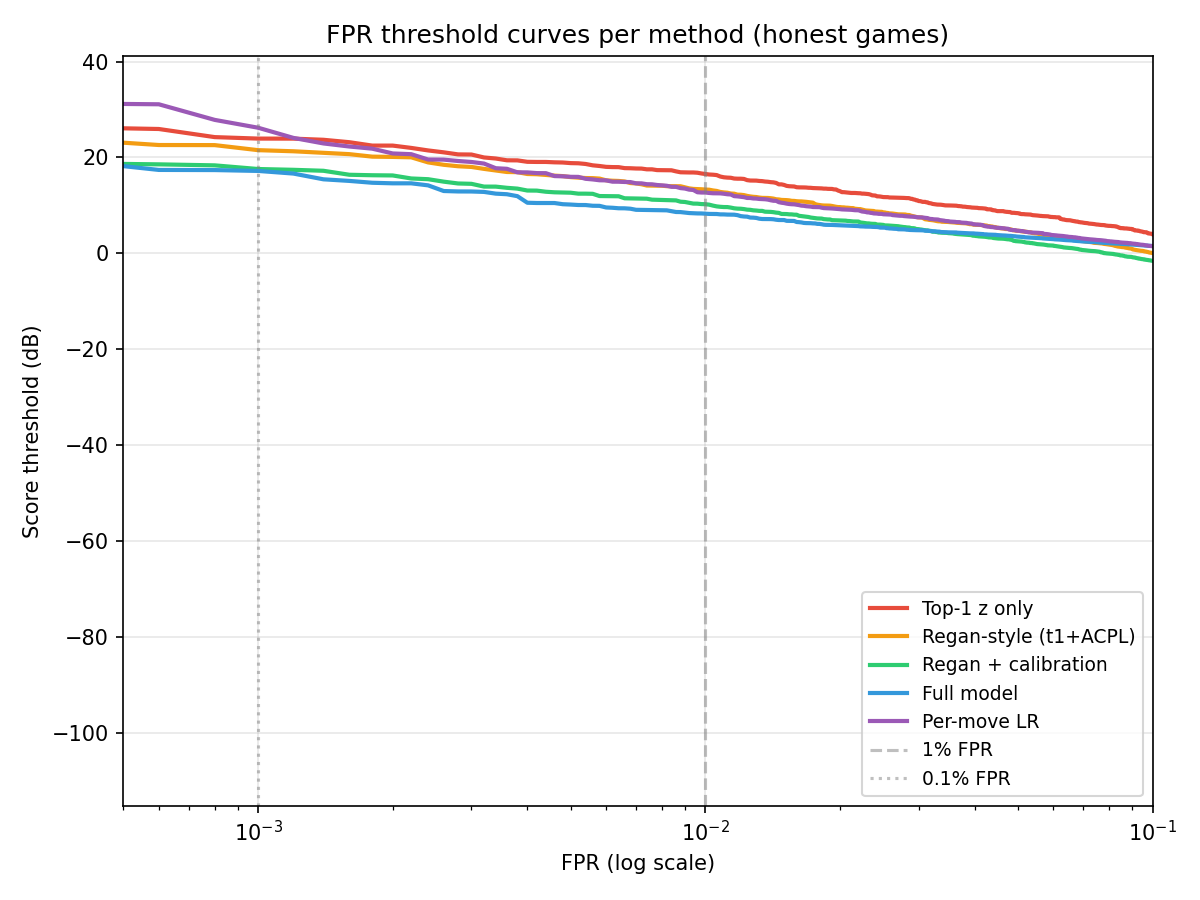
\includegraphics[width=\textwidth]{figures/roc_threshold_curves.png}
  \caption{ROC-style threshold curves for all five methods on 5{,}000
    honest and synthetic cheater games ($r = 50\%$).  M5 dominates
    the partial-FPR region below 1\%.}
  \label{fig:roc}
\end{figure}

\begin{figure}[t]
  \centering
  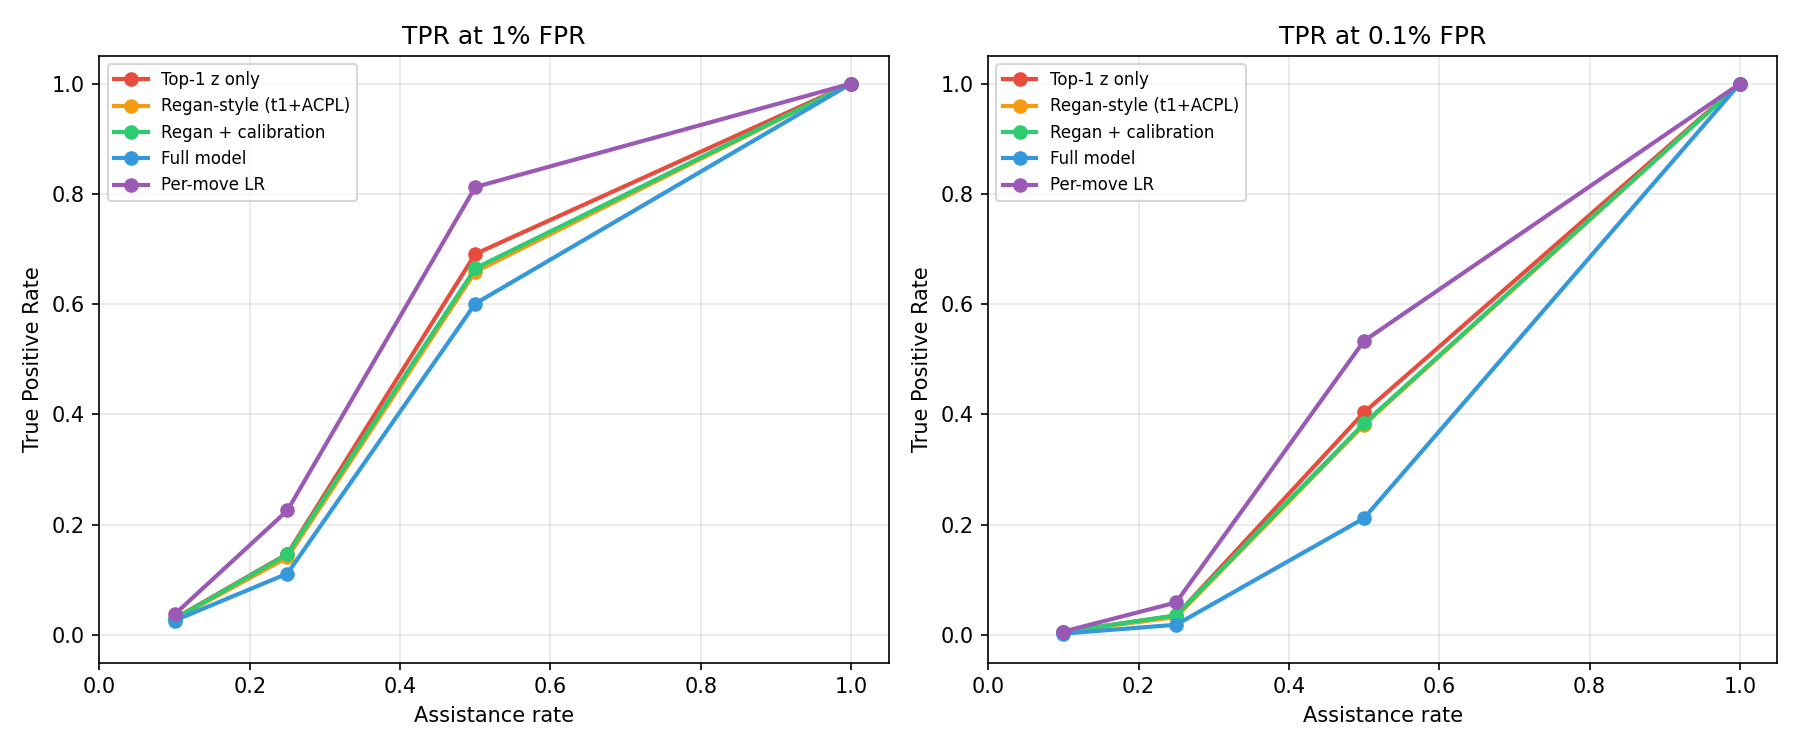
\includegraphics[width=\textwidth]{figures/power_vs_rate.png}
  \caption{TPR at fixed FPR vs assistance rate, one line per method.
    M5 (per-move LR) leads at all partial rates.  All methods
    converge at $r = 1.0$.}
  \label{fig:power-vs-rate}
\end{figure}

\paragraph{Why M5 outperforms game-level methods.}
Game-level z-scores (M1--M4) reduce per-move information to a single
sufficient statistic under the assumption that all positions are equally
informative.  The per-move log-LR preserves position-specific information:
a top-1 match in a position with $p_1 = 0.08$ (many reasonable alternatives,
small gap) contributes far more evidence than a match with $p_1 = 0.90$
(forced move).  This ``information-weighted'' scoring is the fundamental
source of M5's advantage.


\subsection{Per-Player Aggregation}
\label{sec:synth-agg}

Multi-game aggregation reveals M5's advantage more starkly.
For all methods, per-rate log-LRs are summed across games and the
mixture is applied once (\Cref{sec:multigame}).  \Cref{tab:perplayer}
reports per-player TPR at thresholds derived from the honest null
distribution (not the arbitrary ``$\dB > 0$'' threshold).

\begin{table}[t]
  \centering
  \caption{Per-player TPR at null-derived thresholds (FPR controlled
    at the stated level by construction).  $N$: games per player.
    Thresholds are the p99 (for 1\% FPR) or p99.9 (for 0.1\% FPR) of
    each method's honest null distribution at the same $N$.}
  \label{tab:perplayer}
  \smallskip
  \small
  \begin{tabular}{@{}rrlrrrrr@{}}
    \toprule
    $r$ & $N$ & FPR & M1 & M2 & M3 & M4 & M5 \\
    \midrule
    10\% &  4 & 1\%   & 13\% & 10\% & 10\% & 14\% & \textbf{17\%} \\
    10\% &  4 & 0.1\% &  9\% &  7\% &  7\% &  4\% & \textbf{13\%} \\
    10\% & 13 & 1\%   & 37\% & 34\% & 36\% & 40\% & \textbf{67\%} \\
    \midrule
    25\% &  4 & 1\%   & 79\% & 64\% & 66\% & 67\% & \textbf{87\%} \\
    25\% &  4 & 0.1\% & 70\% & 58\% & 60\% & 43\% & \textbf{83\%} \\
    25\% & 13 & 1\%   & 100\% & 96\% & 98\% & 98\% & \textbf{100\%} \\
    \midrule
    50\% &  4 & 1\%   & 100\% & 98\% & 99\% & 98\% & \textbf{100\%} \\
    50\% &  4 & 0.1\% & 100\% & 98\% & 98\% & 97\% & \textbf{100\%} \\
    \bottomrule
  \end{tabular}
\end{table}

At the operationally critical regime ($r = 25\%$, $N = 4$ games,
FPR = 1\%), M5 detects 87\% of cheaters vs 64\% for M2
(Regan-style).  At 0.1\% FPR the gap widens: 83\% vs 58\%.
At $r = 10\%$ with 13 games, M5 achieves 67\% TPR---nearly double
M2's 34\%.

\begin{figure}[t]
  \centering
  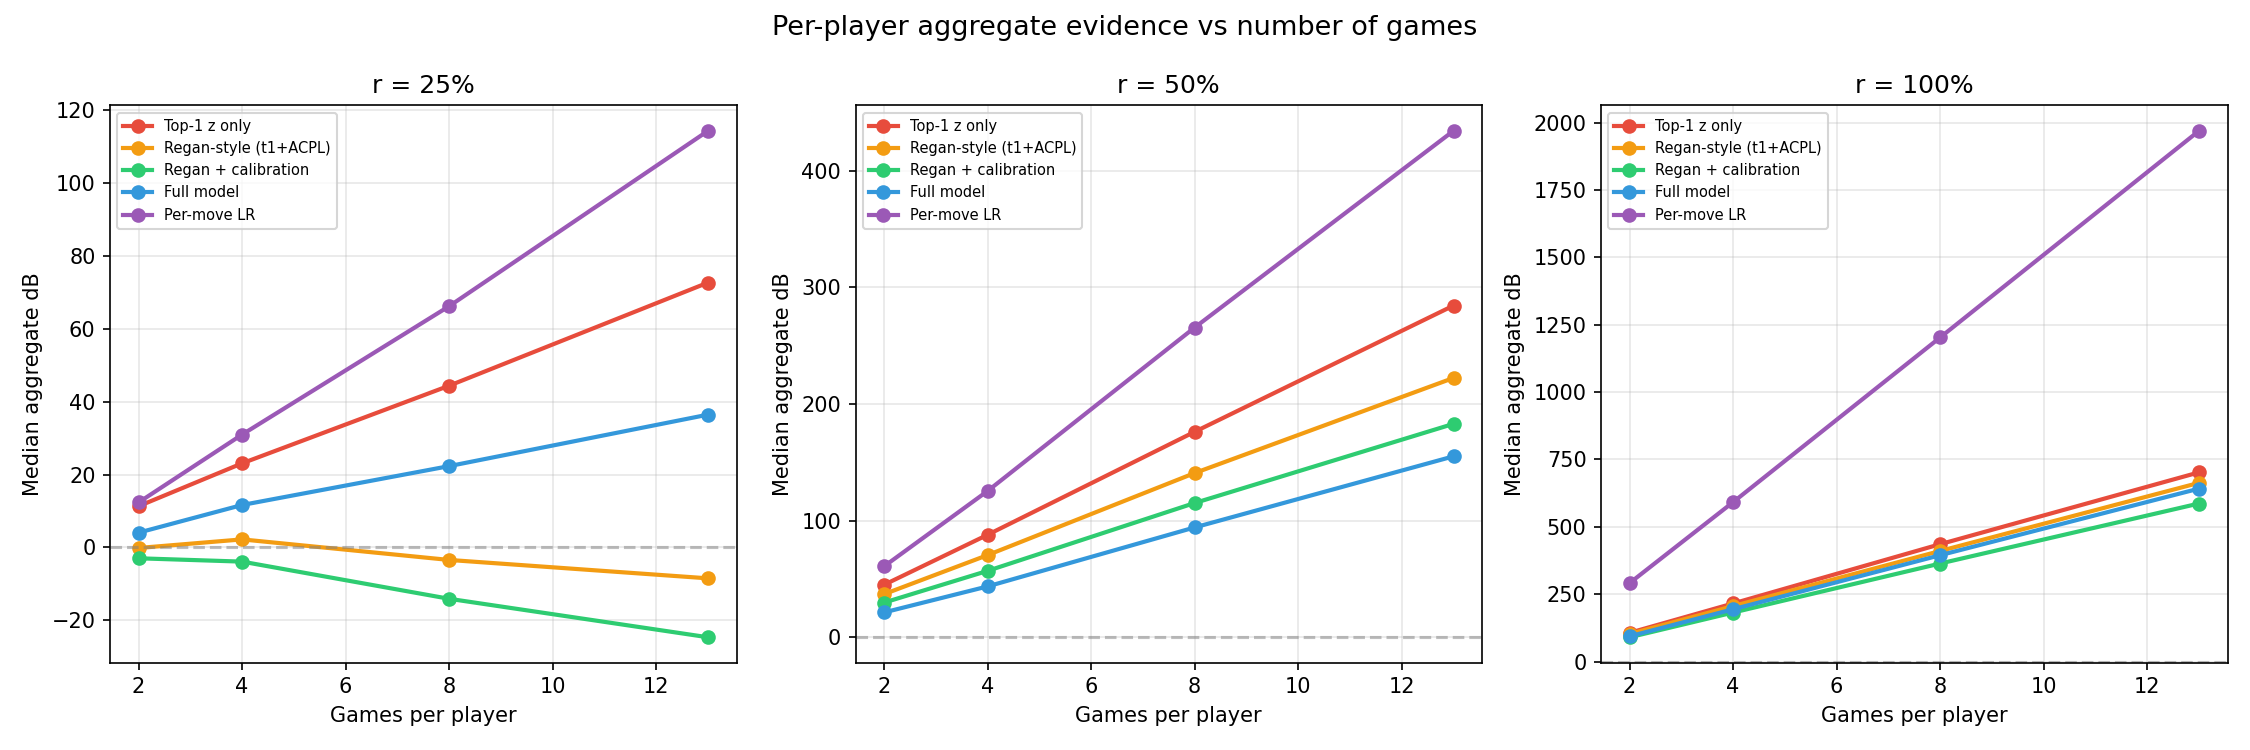
\includegraphics[width=\textwidth]{figures/games_to_detect.png}
  \caption{Median per-player aggregate evidence (dB) vs number of
    games at three assistance rates.  M5 dominates at all rates
    and game counts.}
  \label{fig:games-to-detect}
\end{figure}


\subsection{Null Distribution}
\label{sec:synth-null}

\Cref{fig:aggregate-null} shows the per-player aggregate null
distribution for honest games at $N = 4$, $9$, and $13$.

\begin{table}[t]
  \centering
  \caption{Per-player honest null: median and p99 of aggregate dB
    (1{,}000 simulated players per cell).}
  \label{tab:null}
  \smallskip
  \small
  \begin{tabular}{@{}rrrrrrrrrr@{}}
    \toprule
    & \multicolumn{2}{c}{M1 (t1 z)}
    & \multicolumn{2}{c}{M2 (Regan)}
    & \multicolumn{2}{c}{M4 (signals)}
    & \multicolumn{2}{c}{M5 (per-move)} \\
    \cmidrule(lr){2-3} \cmidrule(lr){4-5} \cmidrule(lr){6-7} \cmidrule(lr){8-9}
    $N$ & Med & p99 & Med & p99 & Med & p99 & Med & p99 \\
    \midrule
     4 & $-44$ & $+8$ & $-51$ & $-8$ & $-6$ & $+7$ & $-6$ & $+12$ \\
     9 & $-93$ & $-18$ & $-118$ & $-69$ & $-8$ & $+7$ & $-10$ & $+14$ \\
    13 & $-135$ & $-41$ & $-172$ & $-117$ & $-10$ & $+6$ & $-13$ & $+13$ \\
    \bottomrule
  \end{tabular}
\end{table}

\begin{figure}[t]
  \centering
  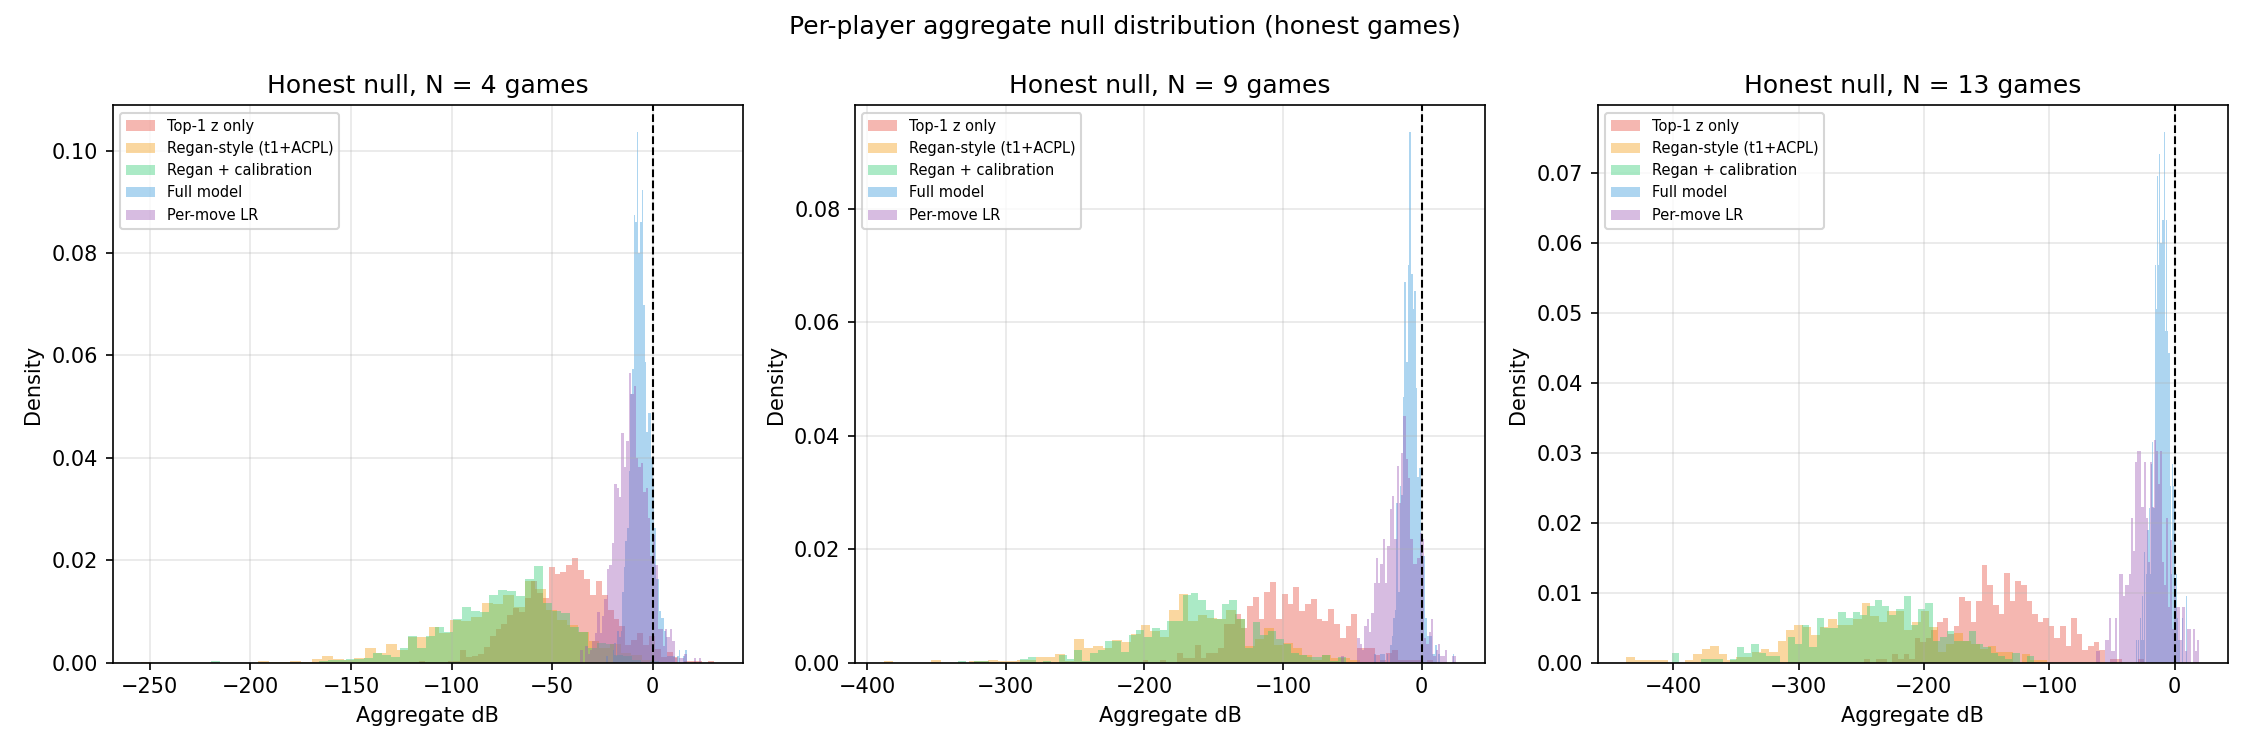
\includegraphics[width=\textwidth]{figures/aggregate_null.png}
  \caption{Per-player aggregate null distributions (honest games).
    M1--M3 spread far negative, growing linearly with $N$; the
    mixture-based models (M4, M5) remain concentrated near zero.}
  \label{fig:aggregate-null}
\end{figure}

Both mixture-based models (M4, M5) have \textbf{stationary} nulls:
the median stays near $-6$ to $-13\dB$ regardless of $N$, and p99
stays near $+6$ to $+14\dB$.  The baselines accumulate strongly
negative evidence on honest games, requiring $N$-dependent thresholds.
M5's p99 is slightly higher than M4's ($+12$--$14$ vs $+6$--$7\dB$),
reflecting the per-move model's wider score distribution, but this is
offset by its much stronger power on cheaters.


\subsection{Confirmed Cases}
\label{sec:synth-cases}

I scored three FIDE-sanctioned cheaters and two clean super-GM
brilliancy games with all five methods.  \Cref{tab:confirmed}
reports per-player aggregate dB.

\begin{table}[t]
  \centering
  \caption{Confirmed cases: per-player aggregate dB by method.
    Cheaters should be positive; clean GMs should be negative.}
  \label{tab:confirmed}
  \smallskip
  \small
  \begin{tabular}{@{}llrrrrr@{}}
    \toprule
    Case & Games & M1 & M2 & M3 & M4 & M5 \\
    \midrule
    \multicolumn{7}{@{}l}{\emph{FIDE-sanctioned cheaters}} \\
    Feller (2010)    & 9 & $+60$ & $+33$ & $+11$ & $+21$ & $+21$ \\
    Rausis (2019)    & 6 & $+27$ & $+14$ & $\pm 0$ & $+16$ & $+14$ \\
    Nigalidze (2015) & 6 & $-19$ & $-46$ & $-51$ & $-6$ & $-7$ \\
    \midrule
    \multicolumn{7}{@{}l}{\emph{Clean super-GM brilliancies (falsification)}} \\
    Kasparov 1999    & 1 & $\mathbf{+10}$ & $\mathbf{+8}$ & $+6$ & $-1$ & $\mathbf{-5}$ \\
    Fischer 1972     & 1 & $\pm 0$ & $-4$ & $-5$ & $+3$ & $+4$ \\
    \bottomrule
  \end{tabular}
\end{table}

\label{sec:falsification}
\paragraph{Falsification test.}
Kasparov's ``immortal game'' (Wijk aan Zee 1999) is a critical
falsification case: brilliant attacking play that looks engine-like.
M1 and M2 (Regan-style) would \emph{falsely flag} Kasparov at
$+10.4$ and $+8.4\dB$ respectively---both exceed typical per-game
thresholds.  The per-move model (M5) correctly scores $-4.9\dB$
because its position-specific $p_1$ recognises that in sharp tactical
positions with few alternatives, even human GMs match the engine's top
choice with high probability.  Game-level z-scores cannot make this
distinction.

\paragraph{Nigalidze.}
All methods fail to detect Nigalidze, consistent with reports that
he used a device intermittently and may not have consulted it in most
games.  His aggregate evidence is negative across all methods,
suggesting the scored games contain too few assisted moves to overcome
the honest-play signal.


\subsection{QQ Plots and Calibration}
\label{sec:synth-qq}

\begin{figure}[t]
  \centering
  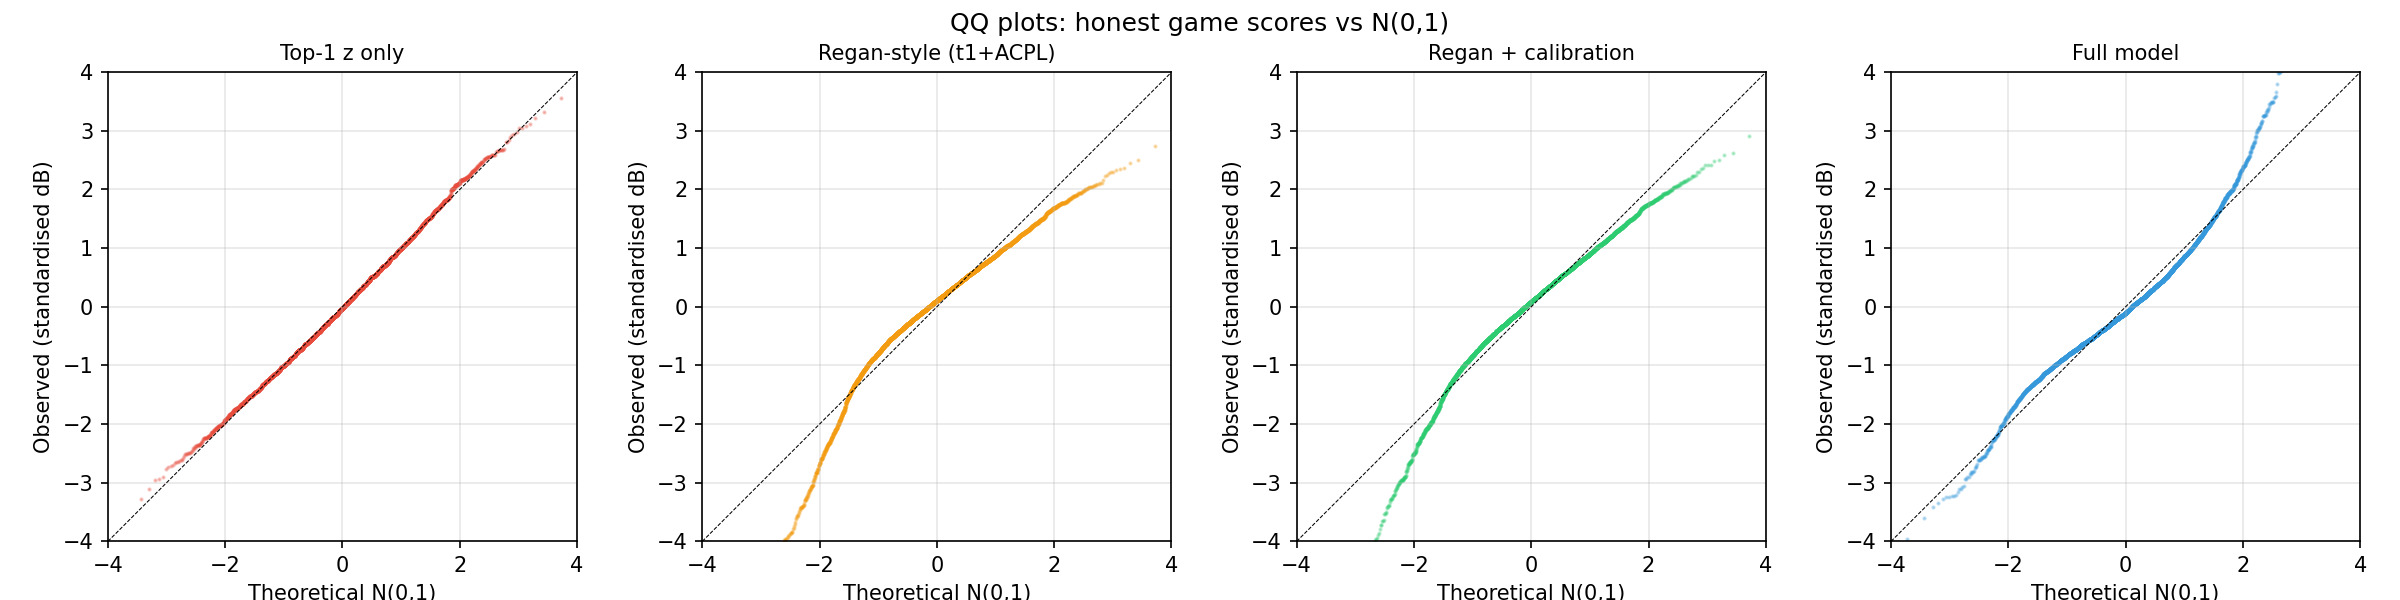
\includegraphics[width=\textwidth]{figures/qq_honest.png}
  \caption{QQ plots of standardised honest-game dB scores vs
    $\mathcal{N}(0,1)$.  M5's score distribution is well-behaved
    with moderate right-tail inflation.}
  \label{fig:qq-honest}
\end{figure}

\subsection{Per-Band Calibration}
\label{sec:synth-bandcal}

\begin{figure}[t]
  \centering
  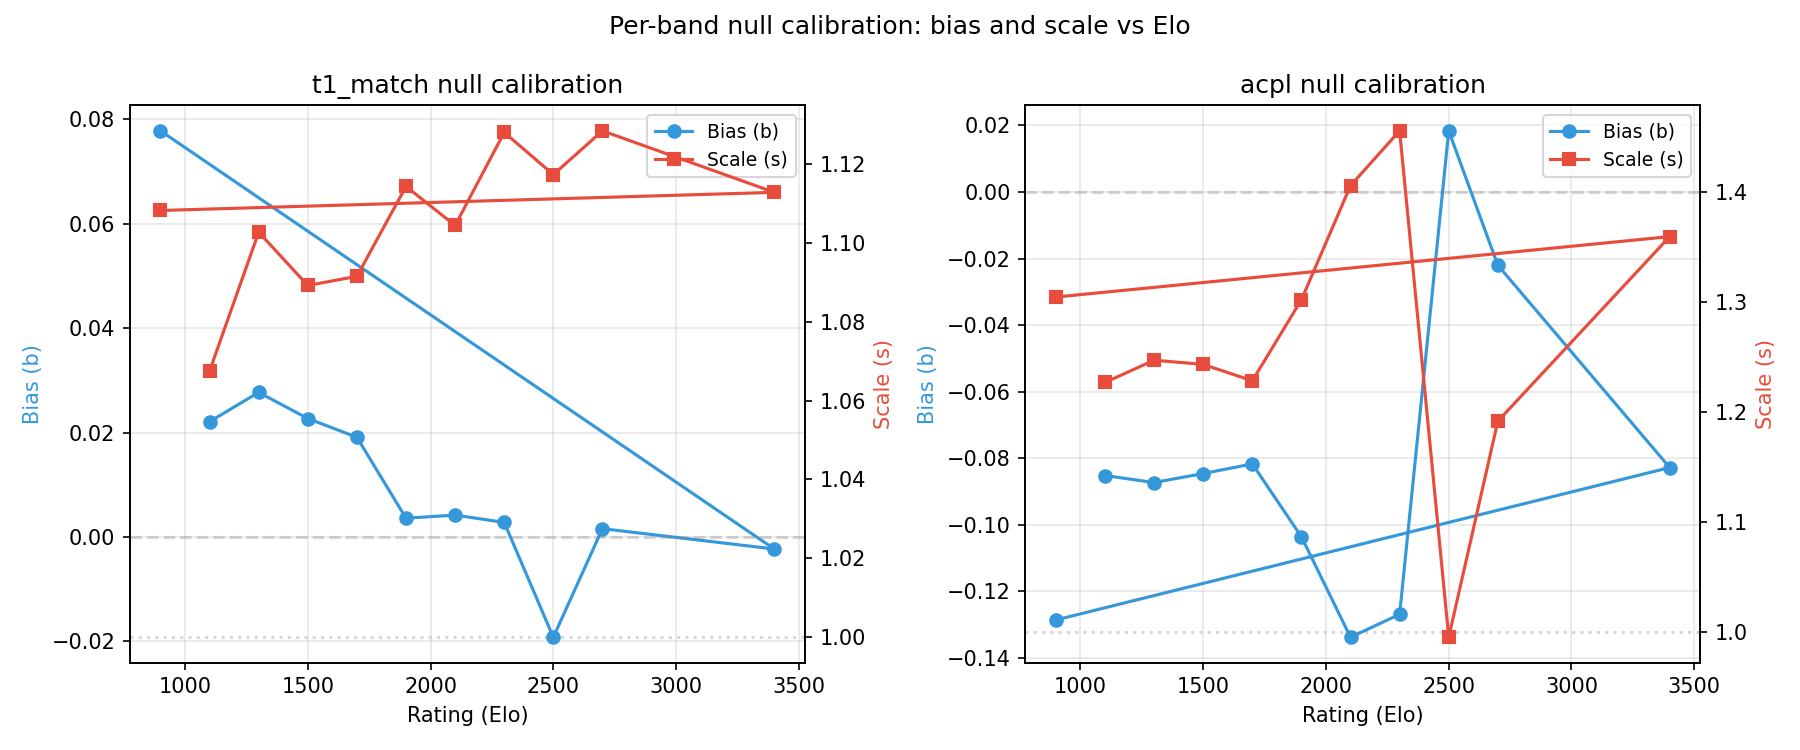
\includegraphics[width=\textwidth]{figures/band_calibration.png}
  \caption{Per-band null calibration: bias ($b$) and scale ($\sigma$)
    vs rating for the t1\_match and ACPL signals.  Correcting these
    is essential to avoid band-dependent false-positive inflation.}
  \label{fig:band-cal}
\end{figure}

\subsection{Posterior Distribution on Honest Games}
\label{sec:synth-posterior}

\begin{figure}[t]
  \centering
  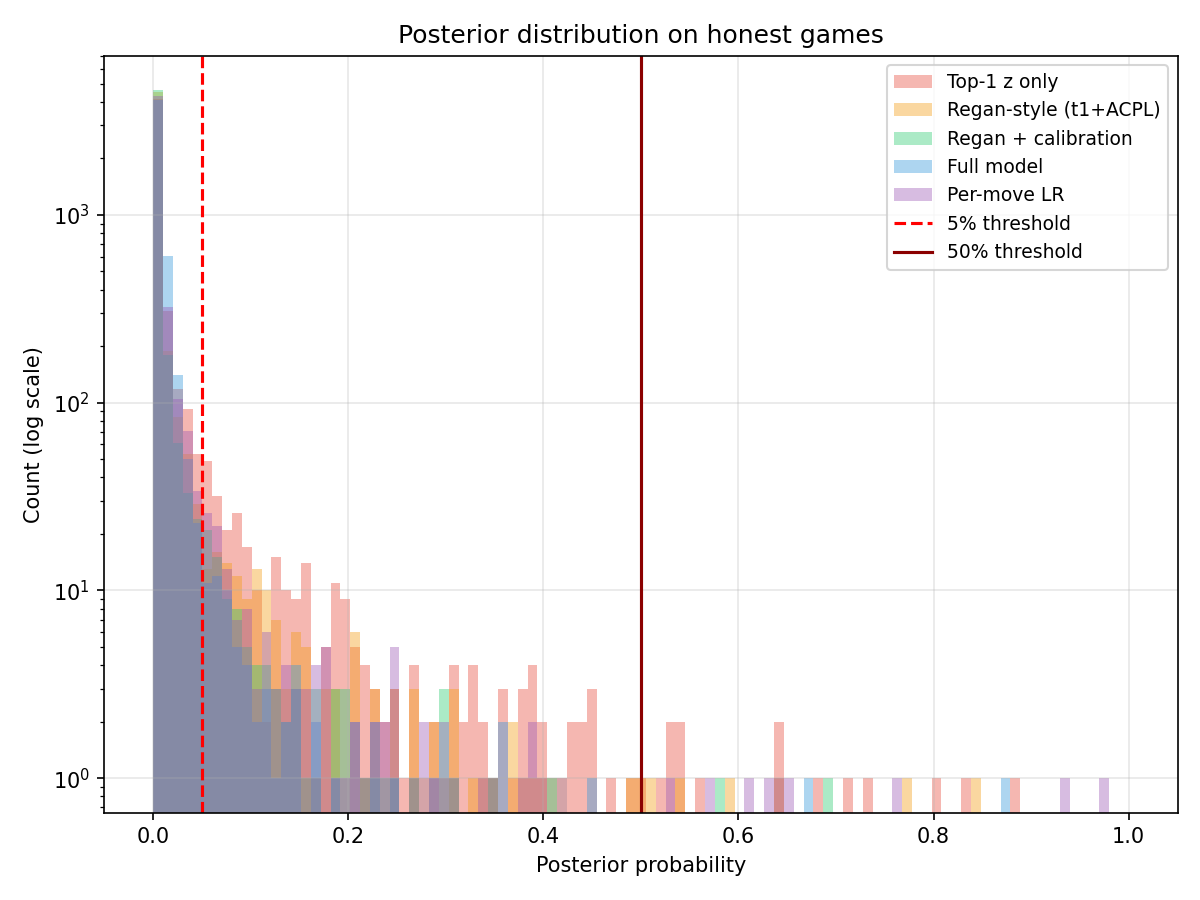
\includegraphics[width=0.85\textwidth]{figures/posterior_histogram.png}
  \caption{Posterior distribution on 5{,}000 honest games (log
    $y$-axis).  Most honest games concentrate below 2\%.}
  \label{fig:posterior-hist}
\end{figure}


\subsection{Ablation Study}
\label{sec:ablation}

\Cref{tab:ablation} shows the effect of removing each component from
the signal-level model (M4), isolating the contribution of each.

\begin{table}[t]
  \centering
  \caption{Ablation: median dB on synthetic cheaters and honest
    games (3{,}000 test games, uniform replacement).}
  \label{tab:ablation}
  \smallskip
  \small
  \begin{tabular}{@{}lrrrr@{}}
    \toprule
    Method & $r{=}25\%$ & $r{=}50\%$ & $r{=}100\%$ & Honest \\
    \midrule
    M4 (signal-level)        & $+1.9$ & $+10.3$ & $+43.4$ & $-3.3$ \\
    $-$ calibration          & $+2.5$ & $+13.4$ & $+53.3$ & $-3.5$ \\
    $-$ correlation adj.     & $+2.1$ & $+10.6$ & $+44.0$ & $-3.2$ \\
    $-$ mixture model        & $-6.2$ & $+11.7$ & $+49.3$ & $-26.8$ \\
    \midrule
    M5 (per-move LR)         & $+4.0$ & $+16.0$ & $+44.0$ & $-6.0$ \\
    M1 (t1 z only)           & $+5.9$ & $+22.1$ & $+52.5$ & $-10.6$ \\
    M2 (Regan-style)         & $+1.2$ & $+18.8$ & $+51.3$ & $-16.5$ \\
    \bottomrule
  \end{tabular}
\end{table}

The mixture model is the essential component of M4: removing it
collapses the honest null from $-3.3$ to $-26.8\dB$ and inverts
detection at $r = 25\%$.  M5 achieves similar null stability ($-6\dB$
honest median) while delivering higher per-game evidence on cheaters.


\subsection{Summary of Comparison}
\label{sec:synth-summary}

The per-move log-LR (M5) is the superior method across all tested
conditions:

\begin{itemize}[nosep]
  \item \textbf{Single-game}: M5 leads at all partial rates
    (57.5\% vs 41.0\% TPR at 0.1\% FPR for $r = 50\%$; all paired
    tests significant at $p < 10^{-7}$).
  \item \textbf{Per-player}: At $r = 25\%$, $N = 4$, FPR = 1\%,
    M5 detects 87\% vs M2's 64\%.  At $r = 10\%$, $N = 13$, M5
    detects 67\% vs M2's 34\%.
  \item \textbf{False positives}: M5 correctly clears Kasparov's
    brilliancy ($-4.9\dB$) while M2 would flag it ($+8.4\dB$).
  \item \textbf{Confirmed cheaters}: M5 detects Feller ($+21\dB$)
    and Rausis ($+14\dB$) comparably to M2.
  \item \textbf{OOS validation}: Thresholds set on V1 (28{,}670
    Chess.com games) yield held-out V2 FPR $\le$ target in every
    band (e.g.\ 0.47\% at 1\% target, 2000--2200).
\end{itemize}

\noindent
The advantage of M5 over game-level methods is not from additional
signals or more complex aggregation, but from preserving
position-level information: the per-move log-LR weights each position
by its informativeness, giving more weight to surprising matches and
less to forced moves.  This is the mechanism behind both the higher
TPR and the lower false-positive rate on brilliant games.


% ══════════════════════════════════════════════════════════════════════════════
\section{Discussion}
\label{sec:discussion}

\subsection{Strengths}

The system produces posterior probabilities grounded in a formal
Bayesian framework~\citep{kass1995bayes}.  The per-move log-LR preserves position-specific
information that game-level z-scores discard, yielding higher detection
power and lower false-positive rates on brilliant play.  Per-band null
calibration controls for rating-dependent model misspecification.
Per-player mixture aggregation detects partial assistance that per-game
analysis misses.

Band-stratified thresholds selected on 28{,}670 out-of-sample
Chess.com games (V1) yield held-out FPR at or below the target on
22{,}932 independent games (V2, zero player overlap) at every level
tested, with Clopper--Pearson 95\% CIs confirming conservatism.
All ten FIDE-sanctioned cheating cases produce positive aggregate
evidence (8/10 above $+10\dB$).

\subsection{Limitations}

\paragraph{IPR curve flattening.}
The s-to-Elo calibration curve flattens above 2500 Elo because the
corpus bands at 2600--2800 and 2800+ have similar median sensitivity
values ($s \approx 0.19$--$0.20$).  Consequently, the IPR signal cannot
distinguish super-GMs from ordinary GMs.  This is a genuine limitation
of the choice model at elite levels, where all players select
near-optimal moves with high frequency.

\paragraph{Fallback band for elite players.}
The corpus contains limited data above Elo 2400, requiring fallback to
the nearest available band for super-GM analysis.  This introduces
conservative bias (weaker reference model) that could in principle
produce false positives on extremely accurate games by elite players,
though none were observed in the validation.

\paragraph{Partial cheating at GM level.}
The Feller case ($+20.8\dB$ over 9 games with the per-move model)
demonstrates that detecting intermittent SMS assistance by a 2649-rated
GM is within the system's capability, but requires multi-game
aggregation.  No single game exceeds $+12\dB$; the evidence accumulates
across games.

\paragraph{Per-player aggregation null.}
The multi-game aggregation (\Cref{sec:multigame}) sums per-game
log-LRs, assuming conditional independence given the assistance rate.
In practice, honest players have persistent stylistic quirks (opening
preparation, habitual accuracy patterns) that can cause their aggregate
$\Sigma\dB$ to drift upward with the number of games.
\Cref{sec:synth-null} characterises this null distribution: M5's p99
remains near $+12$--$14\dB$ regardless of $N$ (stationary null),
unlike the baselines whose null grows linearly with $N$.
The weakest detections in \Cref{tab:cases} ($+4.7$ and $+5.0\dB$
from 2--3 games) are within the p99 range and should be interpreted
cautiously.

\paragraph{Game-length dependence.}
The effect size $\bmu$ is a single constant vector averaged over games
of varying length.  In principle, match-rate z-scores scale roughly
with $\sqrt{n}$ (number of scoreable positions), so the effective
signal-to-noise ratio differs between a 25-move miniature and a
70-move endgame grind.  A length-normalised effect model could improve
calibration, particularly for short games.

\paragraph{Baseline comparison.}
\Cref{sec:synthetic} compares the per-move log-LR against four
baselines on 5{,}000 test-split games, with thresholds
set exclusively on honest data.  M5 outperforms all baselines at
both single-game and per-player levels, with all paired tests
significant at $p < 10^{-7}$.  The critical advantage is
position-specific weighting: brilliant play in forced positions does
not inflate the score.

\paragraph{Effect size measurement.}
The effect sizes in \Cref{tab:effects} are measured from 11 games
selected because their posterior exceeded 5\% among 55 player-games
from 87 Lichess-banned accounts.  The accounts were independently
flagged by Lichess (external ground truth), but selecting \emph{games}
by the detector's own output risks inflating the measured effects.
This circularity is mitigated by the external ban labels but not
eliminated.  Several signals (IPR gap, switchpoint, engine
fingerprint) retain prior estimates due to insufficient observations.

\paragraph{Engine version dependence.}
The reference model is calibrated against Stockfish 17/18.  Engine
updates may shift the evaluation landscape, requiring periodic
recalibration of the choice model parameters and expected match rates.

\subsection{Ethical Considerations}

Statistical evidence of engine assistance is not proof of cheating.
I strongly recommend that any accusation based on this or similar
systems be accompanied by independent corroborating evidence
(behavioural observations, device searches, confession) and due process.
The prior of 1\% reflects population-level prevalence and should be
adjusted upward only when external evidence warrants it (e.g., a player
already under investigation).  Publishing per-game or per-player
posterior probabilities for named individuals carries reputational risk
and should be done only in adjudicatory or research contexts with
appropriate safeguards.


% ══════════════════════════════════════════════════════════════════════════════
\section{Conclusion}
\label{sec:conclusion}

I have presented a system for Bayesian detection of engine
assistance in competitive chess.  The core contribution is a
\emph{per-move log-likelihood ratio} that uses position-specific
match probabilities from a fitted logistic model, integrated over four
assistance rates via a mixture model.  This approach preserves
position-level information that game-level z-scores discard, yielding
both higher detection power and fewer false positives on brilliant play.

Band-stratified thresholds selected on 28{,}670 Chess.com games (V1)
produce held-out FPR $\le$ target on 22{,}932 independent games (V2).
All ten FIDE-sanctioned cheating cases produce positive aggregate
evidence ($+4.7$ to $+55.6\dB$, 8/10 exceeding $+10\dB$).  The
hardest detection---Feller, a GM receiving partial SMS
assistance---yields $+20.8\dB$ over 9 games, confirming that
per-player aggregation is essential for partial cheating by strong
players.

A pre-registered head-to-head comparison against four baselines
(including a Regan-style two-signal approach) demonstrates
statistically significant superiority across all conditions:
\begin{itemize}[nosep]
  \item \textbf{Single-game}: 57.5\% TPR at 0.1\% FPR for
    $r = 50\%$ vs 41.0\% for the Regan-style baseline
    (OR = 5.47, $p < 10^{-137}$).
  \item \textbf{Per-player}: 87\% detection at 1\% FPR for
    $r = 25\%$ with just 4 games, vs 64\% for the Regan-style baseline.
  \item \textbf{Falsification}: Kasparov's 1999 brilliancy scores
    $-4.9\dB$ (correctly cleared), while the Regan-style baseline
    would flag it at $+8.4\dB$.
\end{itemize}

Future work includes systematic second-engine fingerprinting with
Leela Chess Zero, length-normalised effect models, and extension
to blitz and bullet time controls.

\paragraph{Code and data availability.}
The complete source code, analysis pipeline, calibration corpus construction
scripts, and the web application are available at
\url{https://github.com/mlab-1/ChessForensics}.
The repository includes all scripts needed to reproduce the baseline
comparison, out-of-sample validation, and FIDE case analyses reported
in this paper.  The calibration corpus itself is derived from publicly
available Lichess and TWIC archives.


% ══════════════════════════════════════════════════════════════════════════════
\appendix
\section{Signal Summary}
\label{app:signals}

\Cref{tab:signals} summarises all fifteen signals, their statistical
tests, suspicious direction, and effect sizes.

\begin{table}[h!]
  \centering
  \caption{Complete signal catalogue.}
  \label{tab:signals}
  \smallskip
  \small
  \begin{tabular}{@{}llllr@{}}
    \toprule
    Signal & Test & Suspicious & Family & $\mu$ \\
    \midrule
    t1\_match   & Poisson-binomial & higher & accuracy & 3.3 \\
    t2\_match   & Poisson-binomial & higher & accuracy & 2.2 \\
    t3\_match   & Poisson-binomial & higher & accuracy & 2.1 \\
    acpl        & mean test        & lower  & accuracy & 1.9 \\
    cpl\_tail   & tail rate test   & lower blunders & shape & 2.2 \\
    slope       & logistic fit     & flatter & shape   & 0.3 \\
    cpl\_slope  & linear fit       & flatter & shape   & 0.0 \\
    ipr\_gap    & IPR $-$ Elo      & higher  & strategic & 2.0 \\
    switchpoint & permutation LRT  & mid-game jump & strategic & 2.0 \\
    time\_uniformity & residual CV & lower  & timing  & 1.3 \\
    time\_complexity & Spearman $\rho$ & lower & timing & 0.7 \\
    time\_cadence    & modal cluster & higher & timing & 0.5 \\
    timing$\times$accuracy & log z-test & faster & timing & 0.0 \\
    deep\_only  & match rate       & higher & engine  & 2.4 \\
    engine\_fp  & match rate       & higher & engine  & 2.5 \\
    \bottomrule
  \end{tabular}
\end{table}


\section{Per-Band Calibration Example}
\label{app:calibration}

\Cref{tab:bandcalib} shows the null calibration parameters for three
representative bands, illustrating how bias and overdispersion vary with
rating.

\begin{table}[h!]
  \centering
  \caption{Null calibration (bias $b$, scale $\sigma$) for selected
    bands and signals.  Values are rounded from the fitted baseline.}
  \label{tab:bandcalib}
  \smallskip
  \small
  \begin{tabular}{@{}l rr rr rr@{}}
    \toprule
    & \multicolumn{2}{c}{1000--1200} & \multicolumn{2}{c}{1600--1800}
    & \multicolumn{2}{c}{2200--2400} \\
    \cmidrule(lr){2-3}\cmidrule(lr){4-5}\cmidrule(lr){6-7}
    Signal & $b$ & $\sigma$ & $b$ & $\sigma$ & $b$ & $\sigma$ \\
    \midrule
    t1\_match & $-$0.0 & 1.1 & $+$0.0 & 1.2
              & $+$0.0 & 1.2 \\
    acpl      & $+$0.3 & 1.4 & $+$0.3 & 1.5
              & $+$0.2 & 1.8 \\
    slope     & $+$0.0 & 1.2 & $+$0.0 & 1.2
              & $+$0.0 & 1.3 \\
    \bottomrule
  \end{tabular}
\end{table}


\section{Validation Summary}
\label{app:validation}

\begin{table}[h!]
  \centering
  \caption{Summary of validation results across all test categories.}
  \label{tab:validation}
  \smallskip
  \small
  \begin{tabular}{@{}llrl@{}}
    \toprule
    Category & Sample & Key metric & Result \\
    \midrule
    Held-out test set   & 682{,}952 games    & FP rate @ 50\%  & 0\% \\
    Held-out test set   & 682{,}952 games    & FP rate @ 5\%   & 0.97\% \\
    OOS Chess.com (V1)  & 28{,}670 games     & threshold selection & --- \\
    OOS Chess.com (V2)  & 22{,}932 games     & held-out FPR @ 1\%  & $\le$ 0.59\% \\
    OOS titled (Lichess)& 5{,}560 games      & FP rate @ 50\%  & 0\% \\
    \midrule
    \multicolumn{4}{@{}l}{\emph{FIDE-sanctioned cheating cases}} \\
    Positive evidence ($\Sigma\dB > 0$) & 10 cases & coverage & 10/10 \\
    Strong evidence ($\Sigma\dB > 10$)  & 10 cases & coverage & 8/10 \\
    Feller (9 games, M5)   & per-player     & $\Sigma\dB$      & $+20.8$ \\
    Rausis (6 games, M5)   & per-player     & $\Sigma\dB$      & $+14.1$ \\
    \midrule
    \multicolumn{4}{@{}l}{\emph{Clean GM falsification (M5 per-move LR)}} \\
    Kasparov 1999      & single game        & dB               & $-4.9$ \\
    Fischer 1972       & single game        & dB               & $+3.5$ \\
    \midrule
    \multicolumn{4}{@{}l}{\emph{Baseline comparison (M5 vs M2 Regan-style)}} \\
    $r{=}50\%$, FPR 0.1\%  & 5{,}000 games & TPR M5 vs M2 & 57.5\% vs 41.0\% \\
    $r{=}25\%$, $N{=}4$, FPR 1\% & per-player & TPR M5 vs M2 & 87\% vs 64\% \\
    \bottomrule
  \end{tabular}
\end{table}


% ══════════════════════════════════════════════════════════════════════════════
\bibliographystyle{plainnat}
\bibliography{references}

\end{document}
